\documentclass{beamer}

% Top-aligning columns within a top-aligned frame
% https://tex.stackexchange.com/questions/16447/beamer-top-aligning-columns-within-a-top-aligned-frame
\makeatletter
\newenvironment{myitemize}{%
   \setlength{\topsep}{0pt}
   \setlength{\partopsep}{0pt}
   \renewcommand*{\@listi}{\leftmargin\leftmargini \parsep\z@ \topsep\z@ \itemsep\z@}
   \let\@listI\@listi
   \itemize
}{\enditemize}
\makeatother  

\usepackage[USenglish]{babel}
\usepackage[utf8]{inputenc}
\usepackage{amssymb, amsmath}
\usepackage{bm}
\usepackage{color}
\usepackage{tikz}
\usepackage{url}

\definecolor{links}{HTML}{2A1B81}
\hypersetup{colorlinks,linkcolor=,urlcolor=links}

\usetheme{Boadilla}

\bibliographystyle{apalike}
% make bibliography entries smaller
%\renewcommand\bibfont{\scriptsize}
% Now get rid of all the colours
\setbeamercolor*{bibliography entry title}{fg=black}
\setbeamercolor*{bibliography entry author}{fg=black}
\setbeamercolor*{bibliography entry location}{fg=black}
\setbeamercolor*{bibliography entry note}{fg=black}

\newcommand{\lnorm}[1]{\left\lVert#1\right\rVert^2}
\newcommand{\norm}[1]{\left\lVert#1\right\rVert}

% and kill the abominable icon
\setbeamertemplate{bibliography item}{}

\begin{document}
\title[DeBERTa]{DeBERTa: Decoding-enhanced BERT with Disentangled Attention}  
\author{Radek Bartyzal}
\date{2. 3. 2021} 
\institute{GLAMI AI}

\frame{\titlepage} 

%--------- END Frame 12 -------------
\begin{frame}{Motivation}

Paper is by Microsoft Research from 2020/2021.
\vfill

\begin{itemize}
\item improved BERT
\item models available through Hugging Face
\item new SOTA in Language Understanding and Lang. Generation downstream tasks as of January 6, 2021
\item faster pre-training = less steps, but less time?
\end{itemize}


\end{frame}
%--------- END Frame 12 -------------
\begin{frame}{BERT}

Transformer + 

\end{frame}
%--------- END Frame 12 -------------
\begin{frame}{DeBERTa changes to BERT}


\textbf{disentangled attention mechanism}: treat content and position information separately

\vfill

\textbf{relative positional encodings} passed to each layer

\vfill

\textbf{enhanced mask decoder}: provide absolute positional encodings right before the last softmax layer decoding the masked words

\vfill

\textbf{Scale invariant Fine Tuning}: perturbe normalized word embeddings = adversarial training = better generalization

\end{frame}
%--------- END Frame 12 -------------
\begin{frame}{Classic attention mechanism}


\begin{figure}[h]
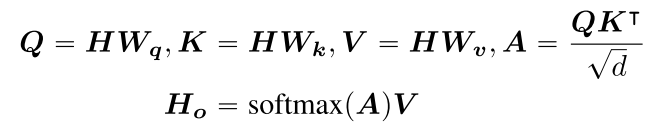
\includegraphics[width=0.6\textwidth]{img/att}
\end{figure}

\begin{itemize}
\item before the first layer word vectors are summed with positional vectors
\item these combined = entangled content vectors are then passed through Transformer layers
\item each layer's attention creates Key, Query and Value vectors from these combined vectors
\end{itemize}

\end{frame}
%--------- END Frame 12 -------------
\begin{frame}{Disentangled attention mechanism}


disentangled attention = at each layer, create separate Key and Query vectors = $K^r$ and $Q^r$ from relative positional vectors 
\begin{figure}[h]
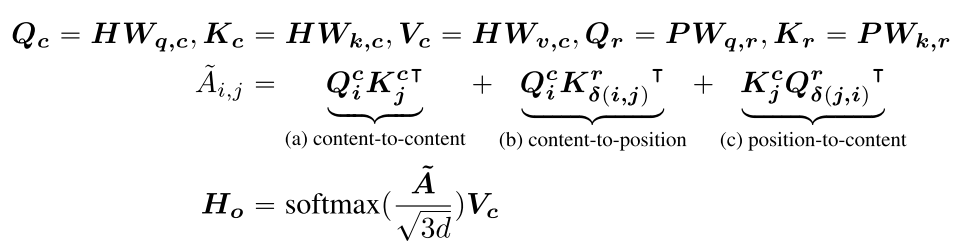
\includegraphics[width=\textwidth]{img/att2}
\end{figure}

\begin{itemize}
\item there is still only one Value vector created from content vector
\item content vectors are the ones transformed by each layer, positional vectors stay the same
\item final attention matrix is sum of attention matrices of possible combinations of Pos. and Content Q/Ks
\end{itemize}

\end{frame}
%--------- END Frame 12 -------------
\begin{frame}{Disentangled attention mechanism}

$P_{i,j}$ = encoding of a position of $i$ relative to $j$
\begin{figure}[h]
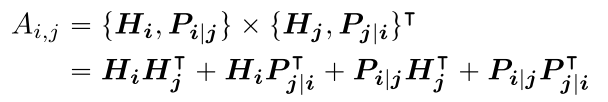
\includegraphics[width=\textwidth]{img/attij}
\end{figure}

Possible attention matrices = combinations of P, C:
\begin{itemize}
\item C to C = classic attention
\item C to P = what relative positions are important to this word
\item P to C = what words are important to these relative positions
\item P to P = what relative position are important to this relative position = does not make sense = not used
\end{itemize}

\end{frame}

%--------- END Frame 12 -------------
\begin{frame}{Disentangled attention: Efficient implementation}

\begin{itemize}
\item an input sequence of length N
\item requires a space complexity of $O(N^2d)$ to store the relative position embedding for each token
\item set the maximum relative distance $k$ to 512 for pre-training
\item embeddings of all possible relative positions are always a subset of $K_r \in R^{2k \times d} \implies$ we can reuse $K_r$ in the attention calculation for all the queries
\item we do not need to allocate memory to store a relative position embedding for each query and thus reduce the space complexity to $O(kd)$ (probably $O(2kd)$) (for storing $K_r$ and $Q_r$)
\end{itemize}



\end{frame}

%--------- END Frame 12 -------------
\begin{frame}{Relative positional encodings}
 
\begin{figure}[h]
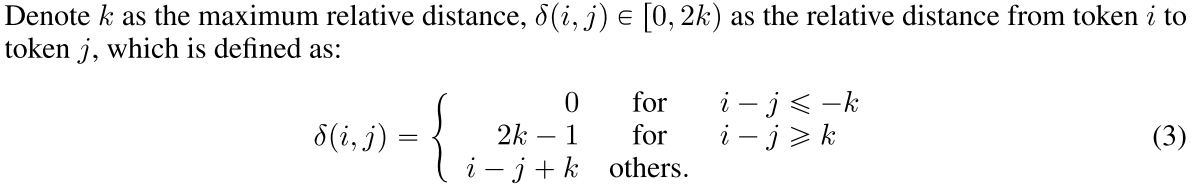
\includegraphics[width=\textwidth]{img/reldist}
\end{figure}

\begin{itemize}
\item the positional vectors are relative = [..., -2, -1, 0, 1, 2, ...]
\item the positional encodings are shared between layers
\item max relative distance = $k=512$, after that just pad: [-2, -2, -1, 0]
\end{itemize}

\end{frame}
%--------- END Frame 12 -------------
\begin{frame}{Scale invariant Fine Tuning = SiFT}

\begin{itemize}
\item The model is regularized: model produces the same output distribution as it produces on an adversarial perturbation of that example.
\item perturbation is applied to the word embedding instead of the word sequence
\item However, the value ranges (norms) of the embedding vectors vary among different words and models.
\item variance gets larger for bigger models with billions of parameters, leading to some instability of adversarial training.
\item SiFT improves the training stability by applying the perturbations to the normalized word embeddings.
\item Specifically, when fine-tuning DeBERTa to a downstream NLP task in our experiments, SiFT first normalizes the word embedding vectors into stochastic vectors, and then applies the perturbation to the normalized embedding vectors. 
\item We find that the normalization substantially improves the performance of the fine-tuned models.
\end{itemize}


\end{frame}

%--------- END Frame 12 -------------
\begin{frame}{Ablation study: everything helps}

\begin{figure}[h]
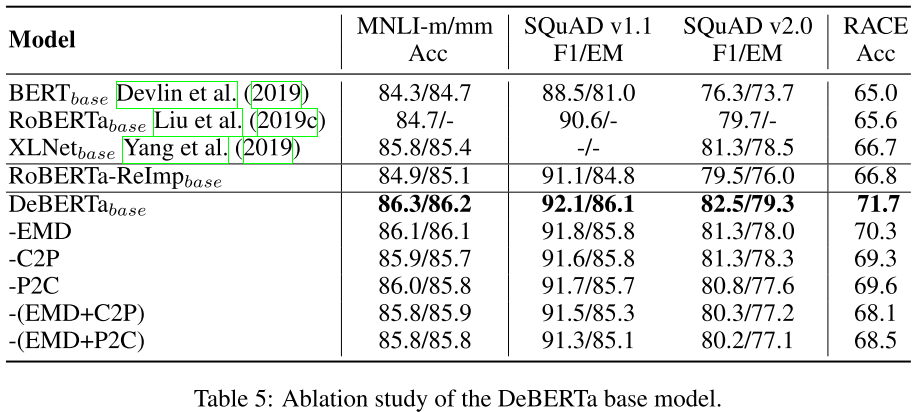
\includegraphics[width=\textwidth]{img/ablation}
\end{figure}

\end{frame}
%--------- END Frame 12 -------------
\begin{frame}{Pre-training needs less steps than RoBERTa}

\begin{figure}[h]
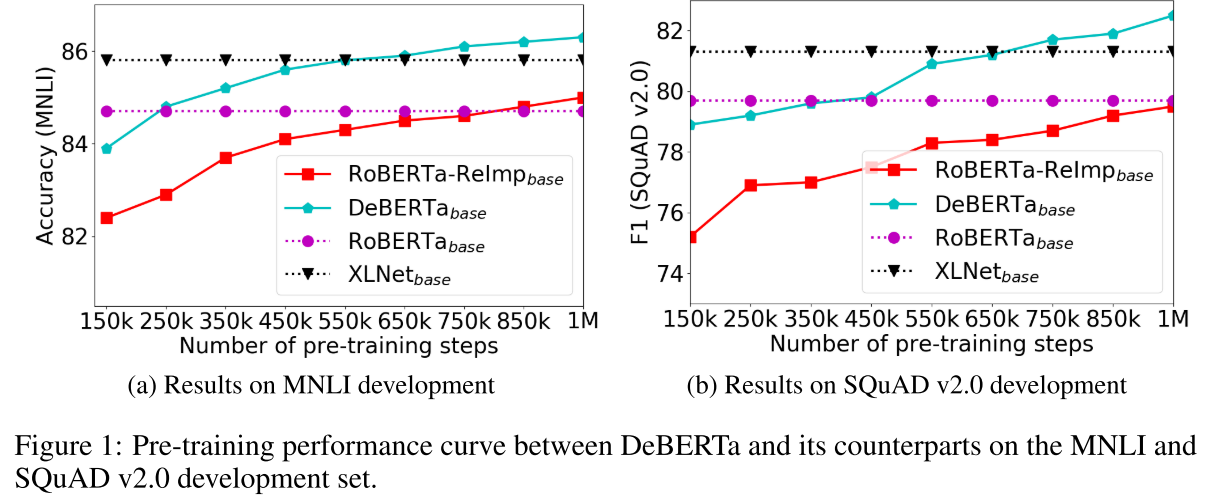
\includegraphics[width=\textwidth]{img/pretraining}
\end{figure}

\end{frame}
%--------- END Frame 12 -------------
\begin{frame}{Results: GLUE}

\begin{figure}[h]
\includegraphics[width=\textwidth]{img/glue}
\end{figure}

We use 6 DGX-2 machines (96 V100 GPUs) to train the models. A single model trained with 2K batch size and 1M steps takes about 20 days.

\end{frame}
%--------- END Frame 12 -------------
\begin{frame}{Results: Comparison with similar sized models}

\begin{figure}[h]
\includegraphics[width=\textwidth]{img/mnli}
\end{figure}

\end{frame}
%--------- END Frame 12 -------------
\begin{frame}{Results: Scale up to 1.5B parameters}

\begin{figure}[h]
\includegraphics[width=\textwidth]{img/superglue}
\end{figure}

\begin{itemize}
\item we share the projection matrices of relative position embedding $W_{k,r},W_{q,}r$ with $W_{k,c},W_{q,c}$, respectively, in all attention layers = not treating the content/positional information differently?
\end{itemize}

\end{frame}
%--------- END Frame 12 -------------
\begin{frame}{Conclusion}

The single 1.5B-parameter DeBERTa model substantially outperforms T5 with 11 billion parameters on the SuperGLUE benchmark by 0.6\%(89.3\% vs. 89.9\%)

\end{frame}


%--------- END Frame 12 -------------
\begin{frame}{Sources}
\begin{thebibliography}{0}

  \bibitem[1]{cit:paper} 1.He, Pengcheng, et al. "Deberta: Decoding-enhanced bert with disentangled attention." arXiv preprint arXiv:2006.03654 (2020). \url{https://arxiv.org/abs/2006.03654} 
  
  
\end{thebibliography}

\end{frame}

 
\end{document}
